\documentclass{article}
\usepackage{graphicx}
\usepackage{ctex}
\usepackage{hyperref}
\usepackage{float}
\usepackage{subfigure}
\usepackage{amsmath}
\usepackage{natbib}
\title{不同分布下的中心极限定理收敛情况以及收敛速度分析}
\author{彭居奕}
\bibliographystyle{plain}
\begin{document}
% \date{2024}
\maketitle
\section{Abstract}
对于不同的\textit{X}的分布以及不同的$\sum_{i=1}^{m}X$对应的\textit{m}值,我们需要精确的指标用于描述\textit{Y}($\sum_{i=1}^{m}X$标准化后的随机变量)的分布与标准正态分布的拟合接近程度,同时有了描述标准之后,我们便可以用与比较不同分布之间的拟合速度。从分布律的角度出发,对于一组数量为$n$的$Y$的频数分布直方图与对应的$n$个标准正态分布变量的理论值进行比较,可以观察到二者在同一横坐标x下的纵坐标总是存在差距,因此可以用频数分布直方图的每一个方块的高度与其理想值的平均距离代表\textit{Y}的拟合表现。根据实验结果,可以证明中心极限定理,同时在实验中比较了各个随机分布的拟合过程特性。所有的实验代码在\url{https://github.com/juyipeng/Central-Limit-Theorem.git}中开源。
\section{Introduction}

对于中心极限定理\cite{laplace}来说,我们知道了当$n\to+\infty$时的极限情况下,Y的分布情况,而且前人已经对其收敛性进行了证明\cite{Liapounov1901}

对于不同的\textit{X}的分布以及不同的$\sum_{i=1}^{m}X$对应的\textit{m}值,我们需要精确的指标用于描述\textit{Y}($\sum_{i=1}^{m}X$标准化后的随机变量)的分布与标准正态分布的拟合接近程度,同时有了描述标准之后,我们便可以用与比较不同分布之间的拟合速度(具体背景见文章的第\ref{cen}部分)。

本文的贡献如下:
\begin{itemize}
\item 提出了拟合损失算法,用于比较Y与标准正态分布的拟合程度
\item 通过实验验证了不同分布下的中心极限定理,并且测定并比较了各自的拟合速度
\end{itemize}



\section{Background}

\subsection{正态分布}
正态分布\cite{gauss},又称高斯分布或常态分布,是极为重要的概率分布,在1809年由德国数学家高斯提出。在特性上,它概率密度函数曲线呈对称钟形,均值、中位数、众数皆为 $\mu$,标准差 $\sigma$ 决定曲线离散程度,$\sigma$ 大则曲线扁平、数据分散,$\sigma$ 小则曲线瘦高、数据集中。应用广泛,工业生产里用于产品质量控制,依均值、标准差设质量标准,保障产品合格率;医学研究中,可研究疾病发病率、药物疗效等分布,预测发病趋势、确定药物适用人群;金融市场内,助经济学家分析金融变量历史数据,预测走势、评估风险,还能构建最优资产组合实现收益风险最优配比。

对正态分布的描述:有随机变量\textit{X},记变量\textit{X}服从于参数为$\mu$、$\sigma^2$的正态分布为$X \sim N(\mu, \sigma^2)$。则有\textit{X}的密度函数为:
\[
f(x) = \frac{1}{\sqrt{2\pi}\sigma}\exp(-\frac{(x-\mu)^2}{2\sigma^2}) \quad -\infty<x<+\infty
\]
正态分布的期望E(X)和方差D(X)分别为:
\begin{flalign*}
&E(X) = \mu \\
&D(X) = \sigma^2
\end{flalign*}


\subsection{几种常见的数据分布}
\subsubsection{均匀分布}
均匀分布是一种连续型变量分布,有随机变量\textit{X},记变量\textit{X}服从于参数为a、b的均匀分布为$X \sim U(a, b)$。则有\textit{X}的密度函数为:
\[
f(x) =
\begin{cases}
1/(b-a) & a<x<b \\
0  & \text{else}
\end{cases}
\]
均匀分布的期望E(X)和方差D(X)分别为:
\begin{flalign*}
&E(X) = (a+b)/2 \\
&D(X) = (b-a)^2/12
\end{flalign*}

\subsubsection{伯努利分布}
伯努利分布是一种离散型随机分布,有随机变量\textit{X},记变量\textit{X}服从于参数为n、p的伯努利分布为$X \sim B(n, p)$。则有\textit{X}的分布律为:
\[
P(X=k)=\frac{n!}{k!(n-k)!}p^k(1-p)^{n-k}
\]
伯努利分布的期望E(X)和方差D(X)分别为:
\begin{flalign*}
&E(X) = np \\
&D(X) = np(1-p)
\end{flalign*}

\subsubsection{泊松分布}
泊松分布是一种离散型随机分布,有随机变量\textit{X},记变量\textit{X}服从于参数为$\lambda$的泊松分布为$X \sim P(\lambda)$。则有\textit{X}的分布律为:
\[
P(X=k)=\frac{e^{-\lambda }\lambda^k}{k!}
\]
泊松分布的期望E(X)和方差D(X)分别为:
\begin{flalign*}
&E(X) = \lambda \\
&D(X) = \lambda
\end{flalign*}

\subsubsection{指数分布}
指数分布是一种连续型变量分布,有随机变量\textit{X},记变量\textit{X}服从于参数为$\lambda$的指数分布为$X \sim E(\lambda)$。则有\textit{X}的密度函数为:
\[
f(x) =
\begin{cases}
\frac{1}{\lambda}\exp(-\frac{x}{\lambda}) & x>0 \\
0  & x<=0
\end{cases}
\]
指数分布的期望E(X)和方差D(X)分别为:
\begin{flalign*}
&E(X) = \frac{1}{\lambda} \\
&D(X) = \frac{1}{\lambda^2}
\end{flalign*}

\subsection{中心极限定理}\label{cen}
中心极限定理\cite{laplace}在1812年由法国数学家拉普拉斯提出,在概率论与数理统计中地位显赫,堪称连接样本统计量与总体参数的关键桥梁,是现代统计学的基石之一。它应用极为广泛,在工业生产里助力质量控制,依据样本测量值判断生产稳定性;于经济金融领域,可剖析市场数据,评估风险、预测趋势;在社会科学研究中,保障抽样调查结果可靠,助力精准计算置信区间。不仅如此,它还与大数定律紧密相连,共同为从样本推断总体筑牢根基,同时为假设检验、置信区间计算提供理论支撑。

中心极限定理的内容如下:假设有$X_1$、$X_2$、$X_3$、...、$X_m$总共m个随机变量属于相同的随机分布且相互独立,且这些变量的期望和方差满足:
\begin{flalign*}
    &E(X_i) = \mu \\
    &D(X_i) = \sigma^2 \\
    & (i = 1,2,3,...,m)
\end{flalign*}
则对于$\sum_{i=1}^{m}X_i$的标准化随机变量$Y=\frac{\sum_{i=1}^{m}X_i - m\mu}{\sigma\sqrt{m}}$ 满足:
\[
\lim_{m\to+\infty}Y \sim N(0,1)
\]

\section{中心极限收敛精度分析}
对于独立同分布的一组随机变量$X_1$、$X_2$、$X_3$、...、$X_m$的和的标准化随机变量$Y=\frac{\sum_{i=1}^{m}X_i - m\mu}{\sigma\sqrt{m}}$来说,由于Y的期望、方差等参数与标准化随机变量完全一致,因此我们想要获取二者的拟合程度,只能从分布律的角度出发。
我们对于一组数量为n的Y的频数分布直方图与对应的n个标准正态分布变量的理论值进行比较,以m=1,n=1000000,$X_i \sim E(0.1)$为例,在图 \ref{comparison1}中,我们可以观察到二者在同一横坐标下的纵坐标总是存在差距。而以m=1000,n=1000000,$X_i \sim E(0.1)$的结果(如图\ref{comparison2})便与理论值几乎完全拟合

\begin{figure}[h]

\subfigure[\footnotesize$m=1$]{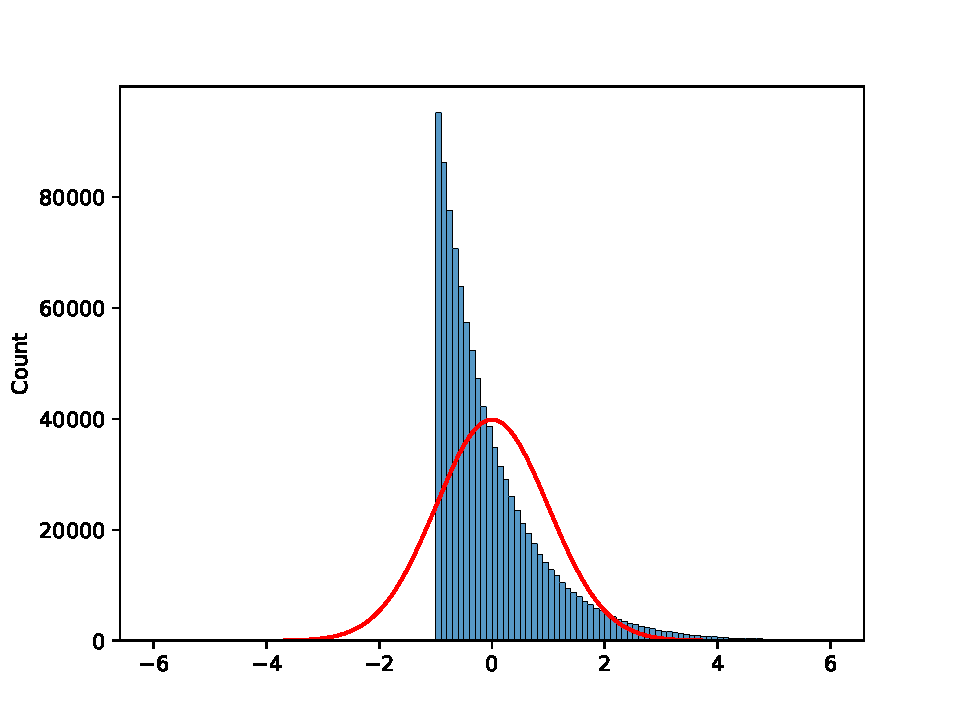
\includegraphics[width = 0.45\textwidth]{../pictures/resfigure_E(0.1)_size1.pdf}\label{comparison1}}
\subfigure[\footnotesize$m=641$]{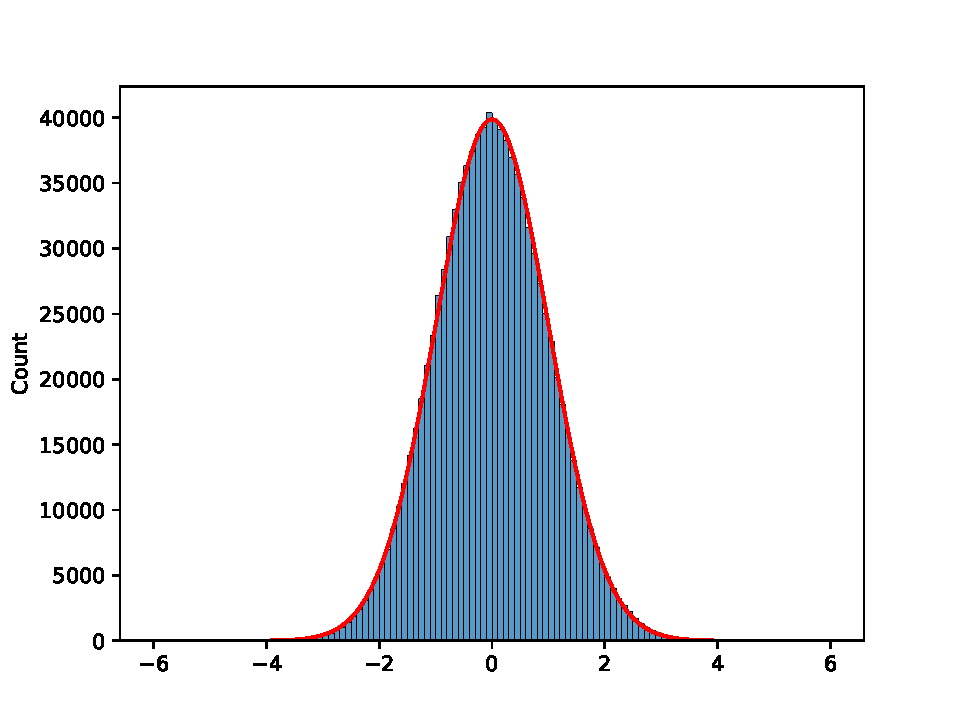
\includegraphics[width = 0.45\textwidth]{../pictures/resfigure_E(0.1)_size1000.pdf}\label{comparison2}}
\caption{\textbf{不同参数 m 的频数直方图,红色曲线代表其在标准正态分布下的理想值}}
\end{figure}




由两张图的对比可知,我们可以用频数分布直方图的每一个方块的高度与其理想值的平均距离代表\textit{Y}的拟合表现。

本文在这里提出拟合损失算法,用于比较Y与标准正态分布的拟合程度:

在x轴上,(-6,6)的区间几乎涵盖了所有的标准正态分布的可能值,将(-6,6)的区间按0.1的宽度划分频数分布直方图,记\textit{R}为改频数分布直方图所有矩形的集合,每一个矩形可看作落在对应区间的\textit{Y}的数量。我们将[a,b]记作此区间的下、上界,h记作矩形的高,代表了落在区间内的数据量。此区间的\textit{Y}的数量的理想值为:
\[
m\cdot\int_{a}^{b}\frac{1}{\sqrt{2\pi}}\exp(-x^2/2)dx
\]
用改理论值与矩形的真实高度h作差,便可以得到理论值和真实值的距离,为了获取更好的拟合效果,将此差值作平方,使得更大的差值对于结果的影响更大,最后便可得到单个方块的Loss值
\[
L_i = (h_i - m\cdot\int_{a_i}^{b_i}\frac{1}{\sqrt{2\pi}}\exp(-x^2/2)dx)^2
\]

对所有的$L_i$求平均,可以得到理论值和真实值的误差平均值,同时,为了获取更好的拟合效果,我们将其取对数,从而可以更好地观察在Loss更小时的特性,最后我们便可以得到最终的Loss值:
\[
Loss = log(\frac{1}{120}\cdot\sum_{i\in R}^{}(h_i - m\cdot\int_{a_i}^{b_i}\frac{1}{\sqrt{2\pi}}\exp(-x^2/2)dx)^2)
\]
此Loss值便可以代表\textit{Y}与标准正态分布的拟合精度。并且二者为负相关,Loss越高,拟合精度越低。





\section{Experiments}\label{experiment}
针对不同的m值和不同的随机分布,进行了一系列的实验。
\subsection{不同随机分布下中心极限定理的验证}
针对不同的随机分布,进行了一系列的实验。对每一种随机分布,我们为其设置合理的参数,然后可以得到其期望和方差,即对应的$\mu\text{和}\sigma$值,通过设置不同的\textit{m}值(即数每一组数据的随机变量个数),我们可以观察到频数分布直方图与理论值的拟合情况。
\subsubsection{均匀分布}
参数设置:
\[
n=1000000, a = -\sqrt{3}, b = \sqrt{3}, \mu = 0, \sigma = 1
\]
实验结果:

画出$m = 1, m = 2, m = 5, m = 10, m = 100, m = 1000$时的频数分布直方图(如图\ref{uni}),从图中可以直观地看到,随着$m$值的升高,$Y$的频数分布直方图不断地拟合接近标准正态分布的理想值。
\begin{figure}[h]

    \subfigure[\footnotesize$m=1$]{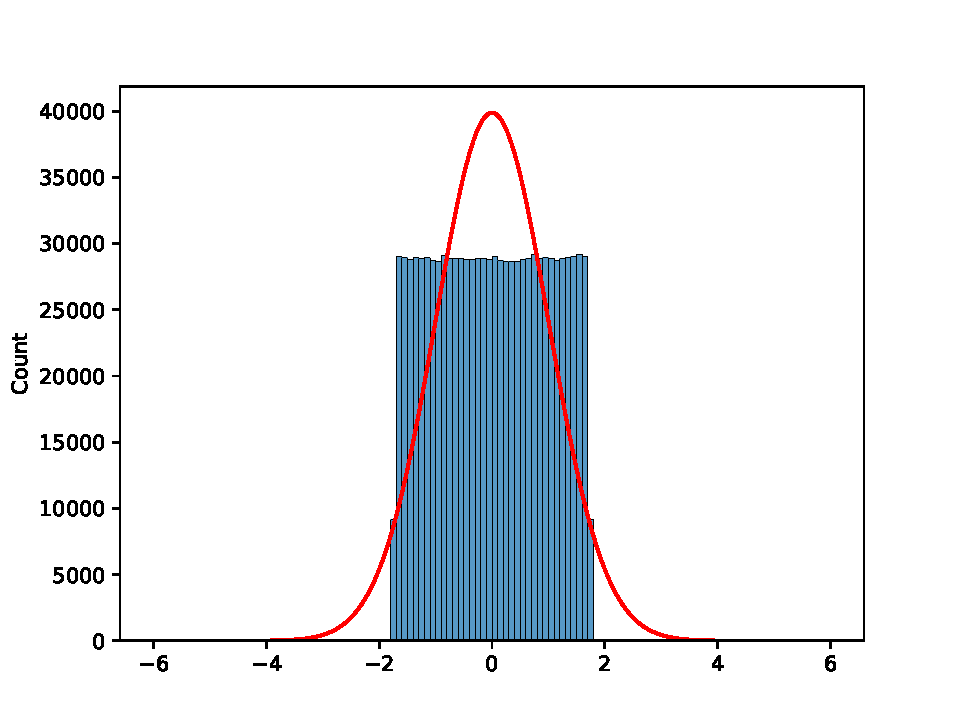
\includegraphics[width = 0.45\textwidth]{../pictures/resfigure_U(-sqrt3_sqrt3)_size1.pdf}}
    \subfigure[\footnotesize$m=2$]{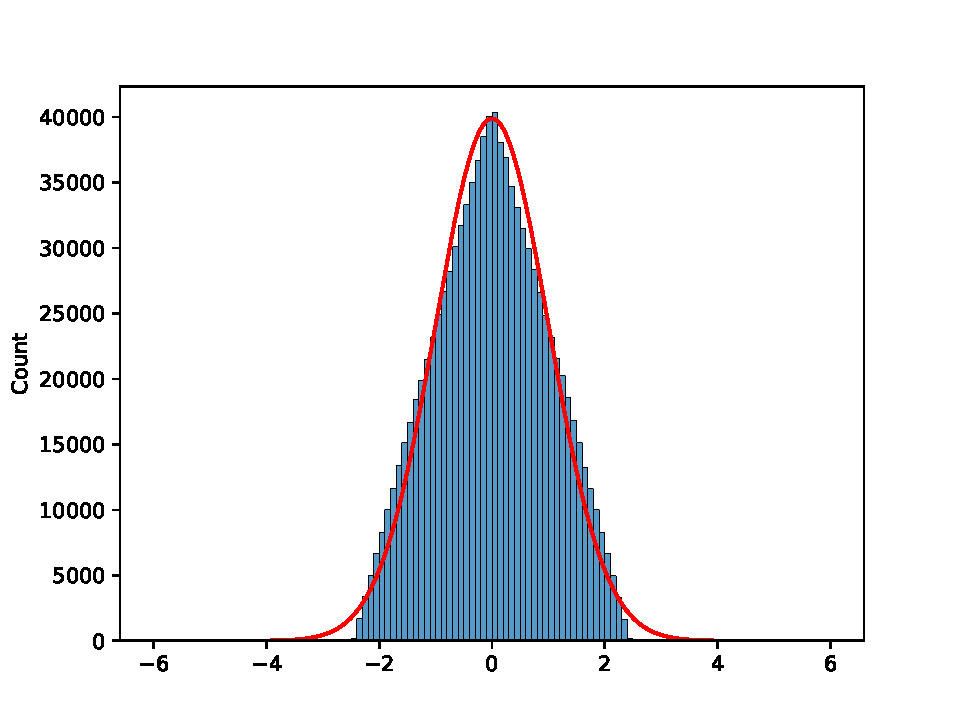
\includegraphics[width = 0.45\textwidth]{../pictures/resfigure_U(-sqrt3_sqrt3)_size2.pdf}}
    \subfigure[\footnotesize$m=5$]{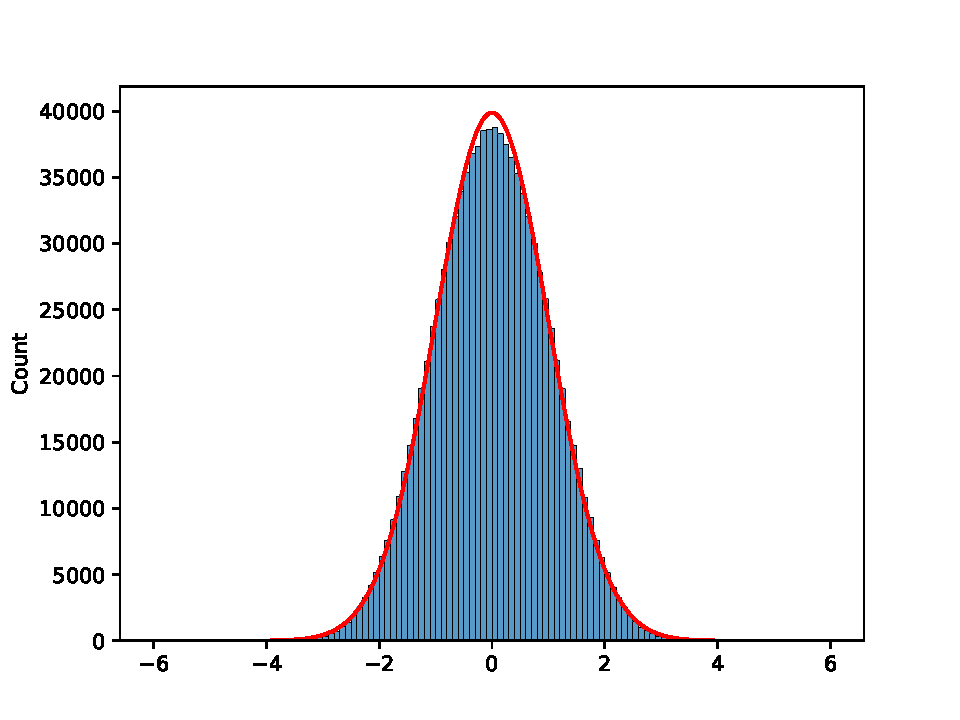
\includegraphics[width = 0.45\textwidth]{../pictures/resfigure_U(-sqrt3_sqrt3)_size5.pdf}}
    \subfigure[\footnotesize$m=10$]{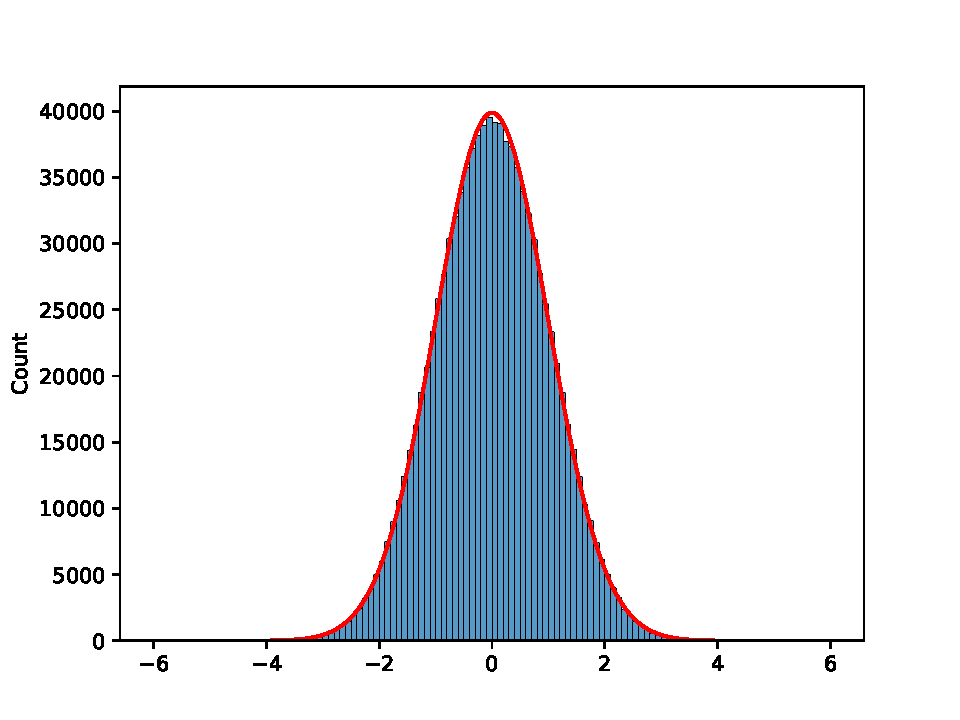
\includegraphics[width = 0.45\textwidth]{../pictures/resfigure_U(-sqrt3_sqrt3)_size10.pdf}}
    \subfigure[\footnotesize$m=100$]{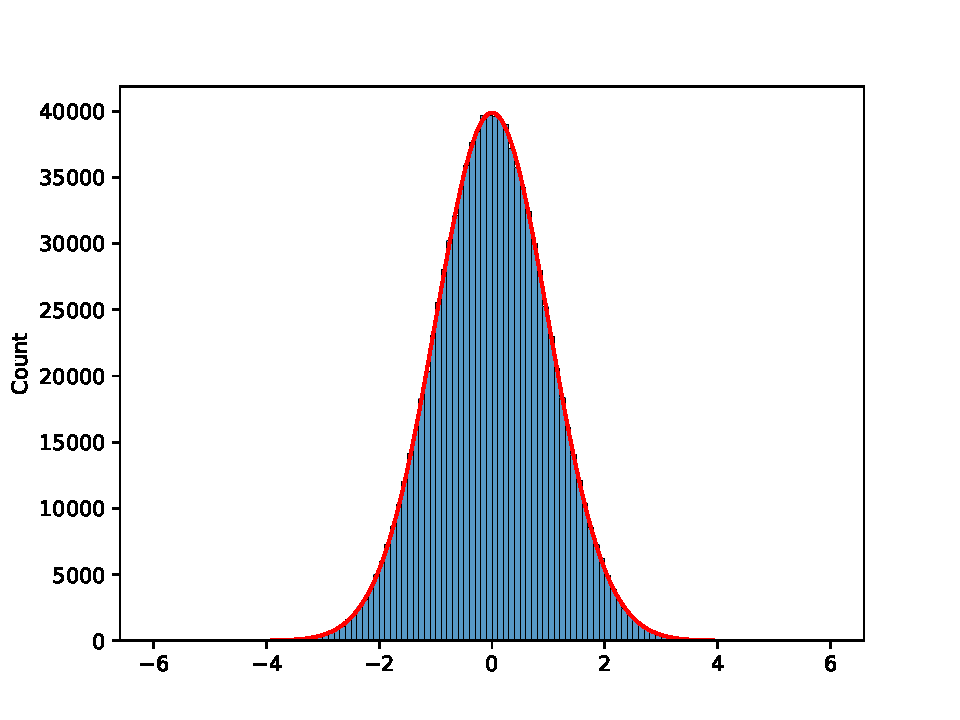
\includegraphics[width = 0.45\textwidth]{../pictures/resfigure_U(-sqrt3_sqrt3)_size100.pdf}}
    \subfigure[\footnotesize$m=1000$]{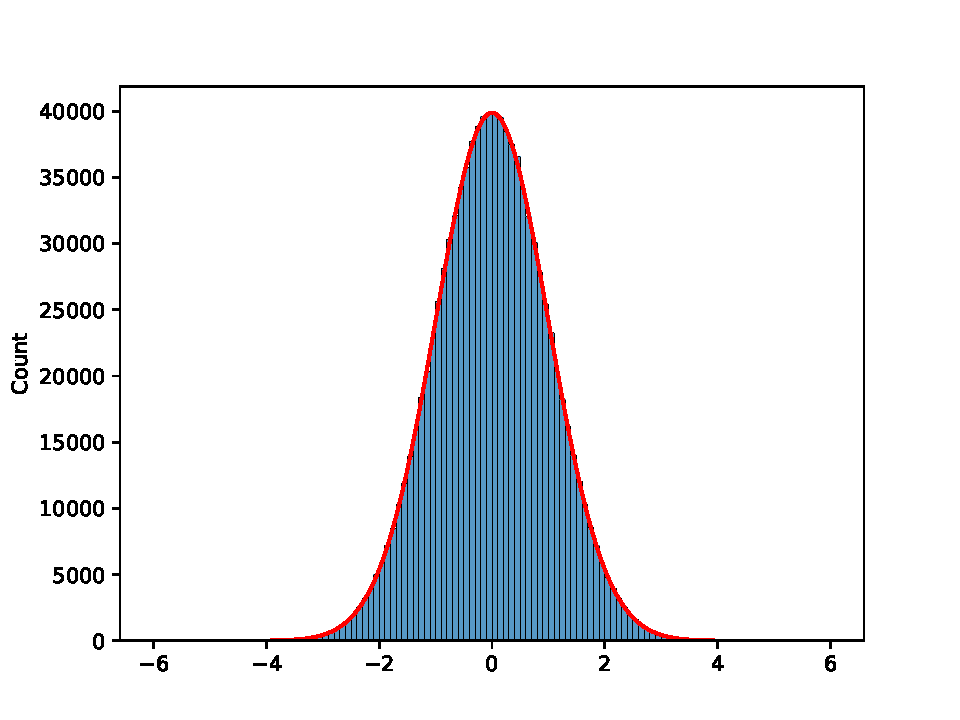
\includegraphics[width = 0.45\textwidth]{../pictures/resfigure_U(-sqrt3_sqrt3)_size1000.pdf}}
    \caption{\textbf{均匀分布下不同$m$值对应的频数分布直方图,红色曲线代表其在标准正态分布下的理想值}}
    \label{uni}
    \end{figure}

\subsubsection{伯努利分布}
参数设置:
\[
n=1000000, n = 100, p = 0.3, \mu = 30, \sigma = \sqrt{21}
\]
实验结果:

画出$m = 1, m = 2, m = 5, m = 10, m = 100, m = 1000$时的频数分布直方图(如图\ref{bo}),从图中可以直观地看到,随着$m$值的升高,$Y$的频数分布直方图不断地拟合接近标准正态分布的理想值。
\begin{figure}[h]

    \subfigure[\footnotesize$m=1$]{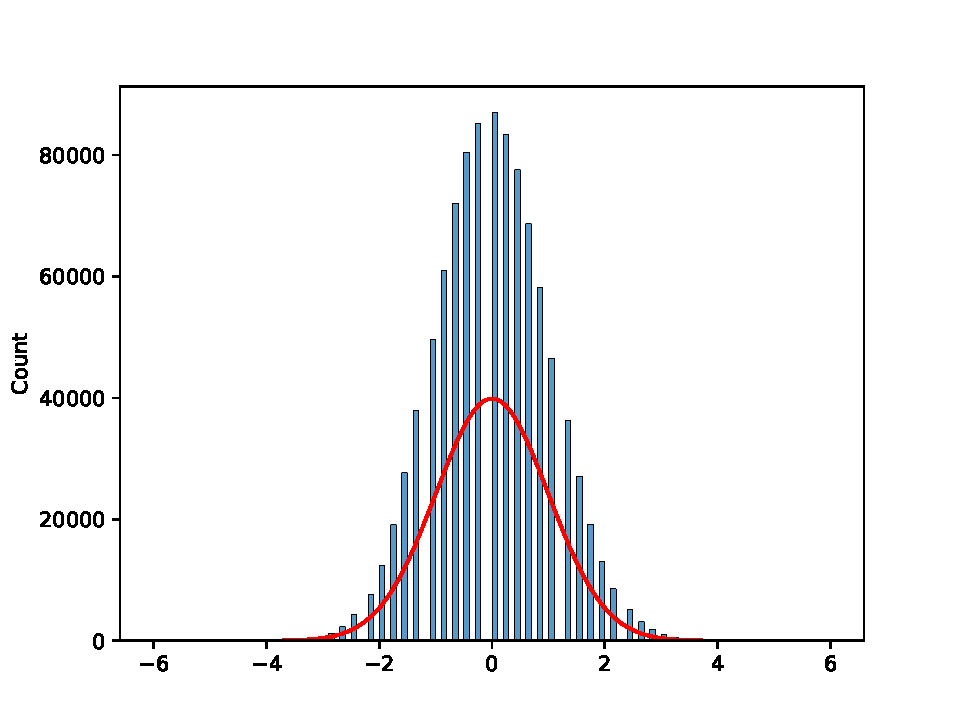
\includegraphics[width = 0.45\textwidth]{../pictures/resfigure_B(100_0.3)_size1.pdf}}
    \subfigure[\footnotesize$m=2$]{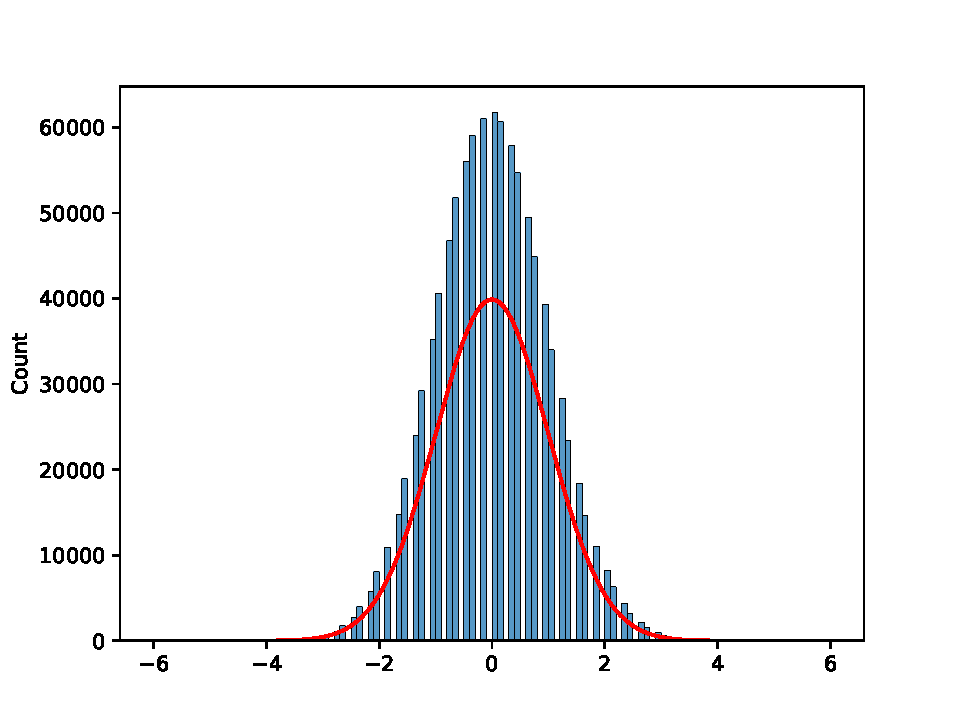
\includegraphics[width = 0.45\textwidth]{../pictures/resfigure_B(100_0.3)_size2.pdf}}
    \subfigure[\footnotesize$m=5$]{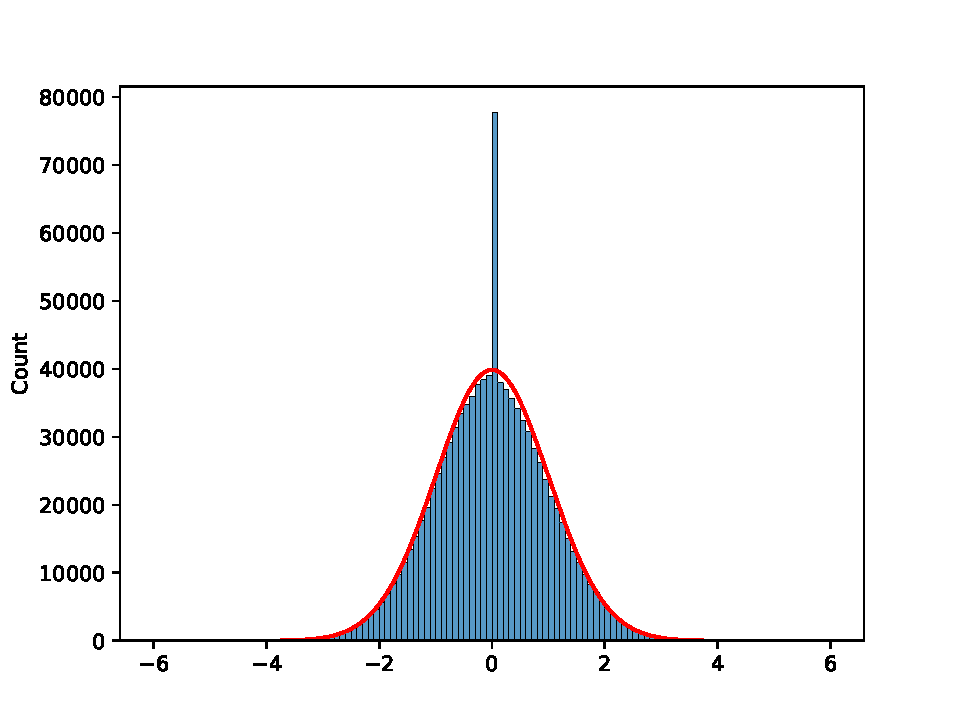
\includegraphics[width = 0.45\textwidth]{../pictures/resfigure_B(100_0.3)_size5.pdf}}
    \subfigure[\footnotesize$m=10$]{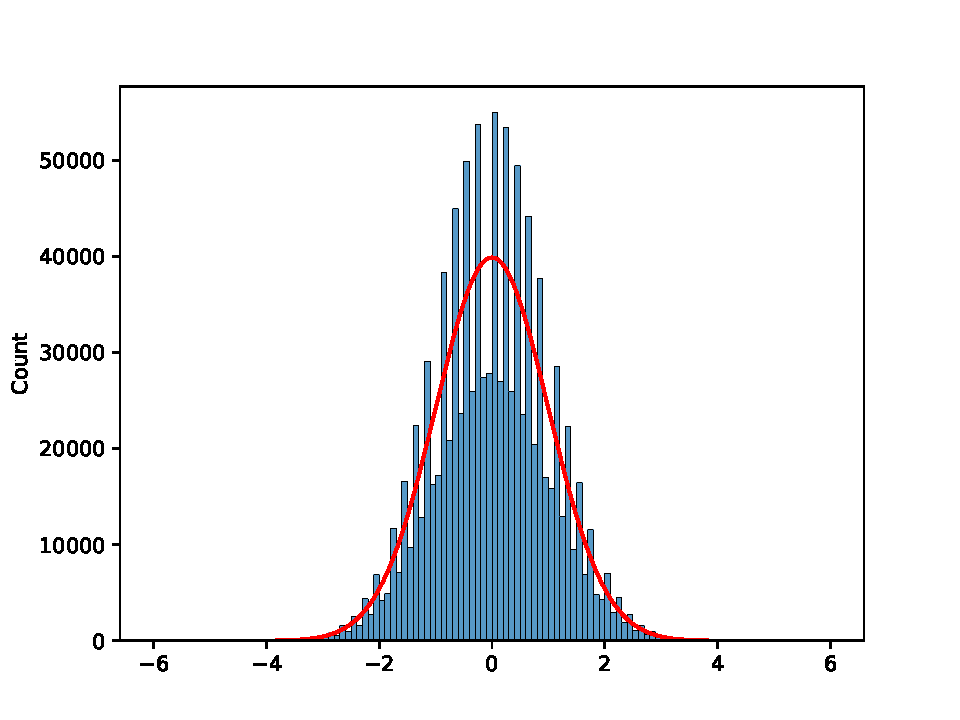
\includegraphics[width = 0.45\textwidth]{../pictures/resfigure_B(100_0.3)_size10.pdf}}
    \subfigure[\footnotesize$m=100$]{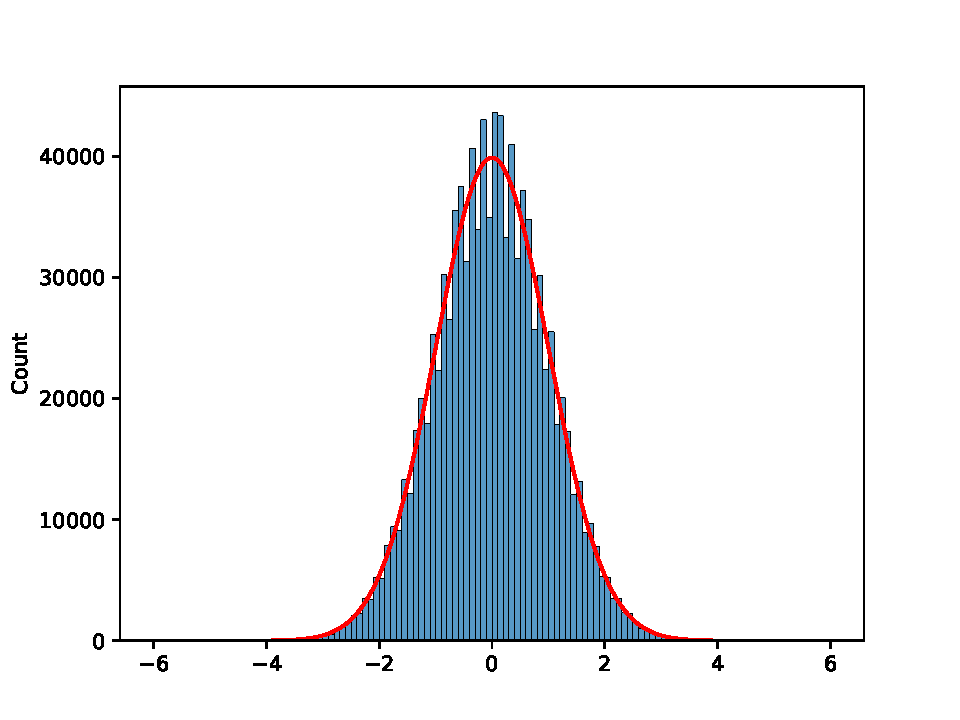
\includegraphics[width = 0.45\textwidth]{../pictures/resfigure_B(100_0.3)_size100.pdf}}
    \subfigure[\footnotesize$m=1000$]{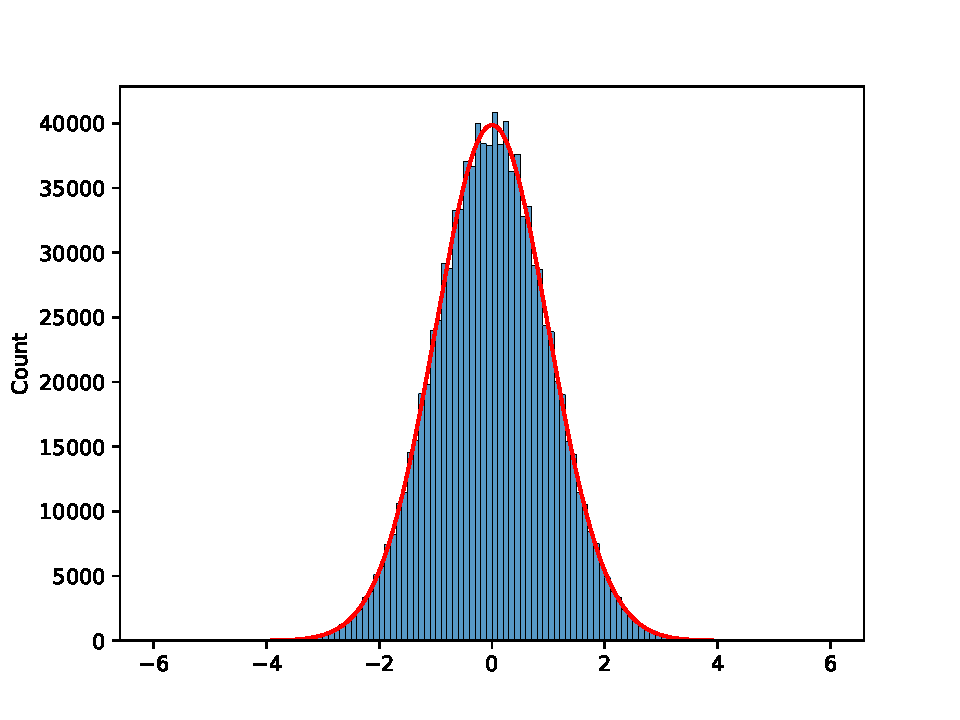
\includegraphics[width = 0.45\textwidth]{../pictures/resfigure_B(100_0.3)_size1000.pdf}}
    \caption{\textbf{伯努利分布下不同$m$值对应的频数分布直方图,红色曲线代表其在标准正态分布下的理想值}}
    \label{bo}
    \end{figure}

\subsubsection{泊松分布}
参数设置:
\[
n=1000000, \lambda = 5, \mu = 5, \sigma = \sqrt{5}
\]
实验结果:

画出$m = 1, m = 2, m = 5, m = 10, m = 100, m = 1000$时的频数分布直方图(如图\ref{poi}),从图中可以直观地看到,随着$m$值的升高,$Y$的频数分布直方图不断地拟合接近标准正态分布的理想值。
\begin{figure}[h]

    \subfigure[\footnotesize$m=1$]{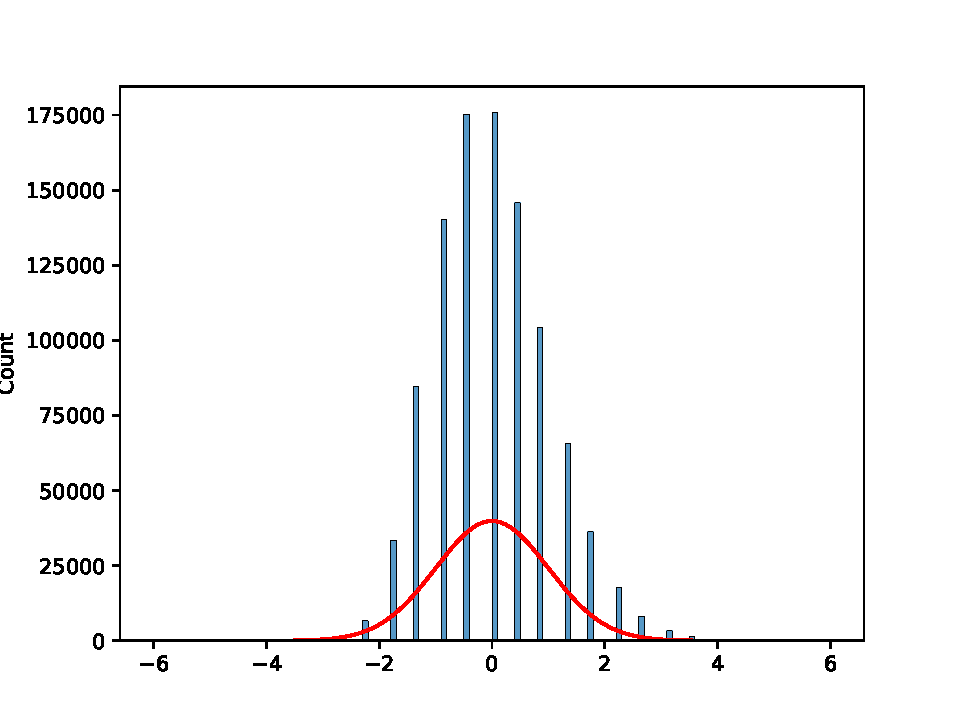
\includegraphics[width = 0.45\textwidth]{../pictures/resfigure_P(5)_size1.pdf}}
    \subfigure[\footnotesize$m=2$]{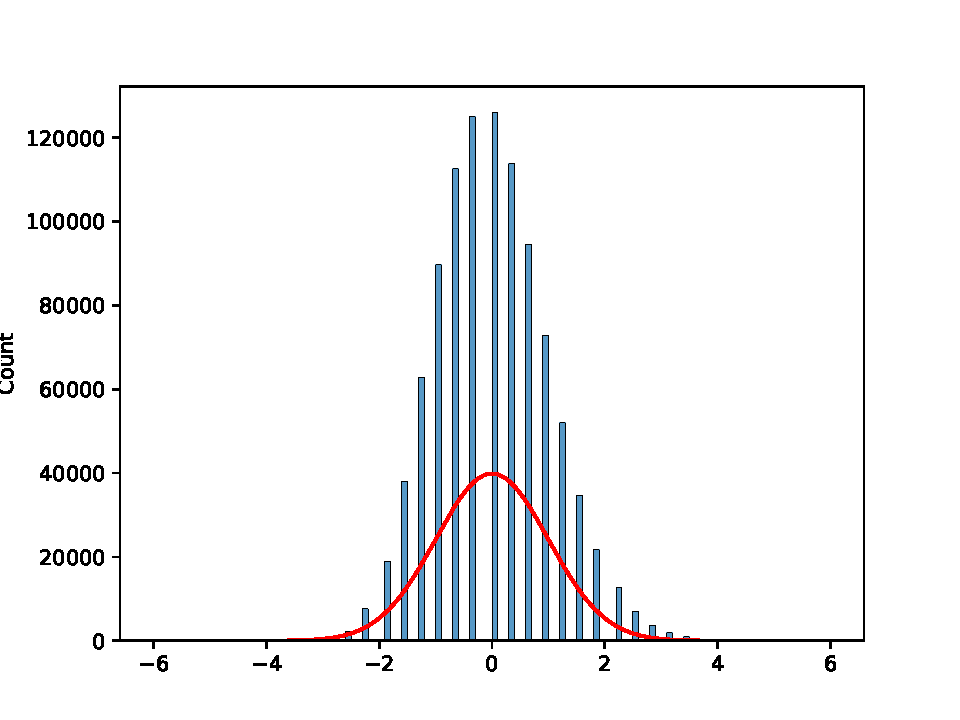
\includegraphics[width = 0.45\textwidth]{../pictures/resfigure_P(5)_size2.pdf}}
    \subfigure[\footnotesize$m=5$]{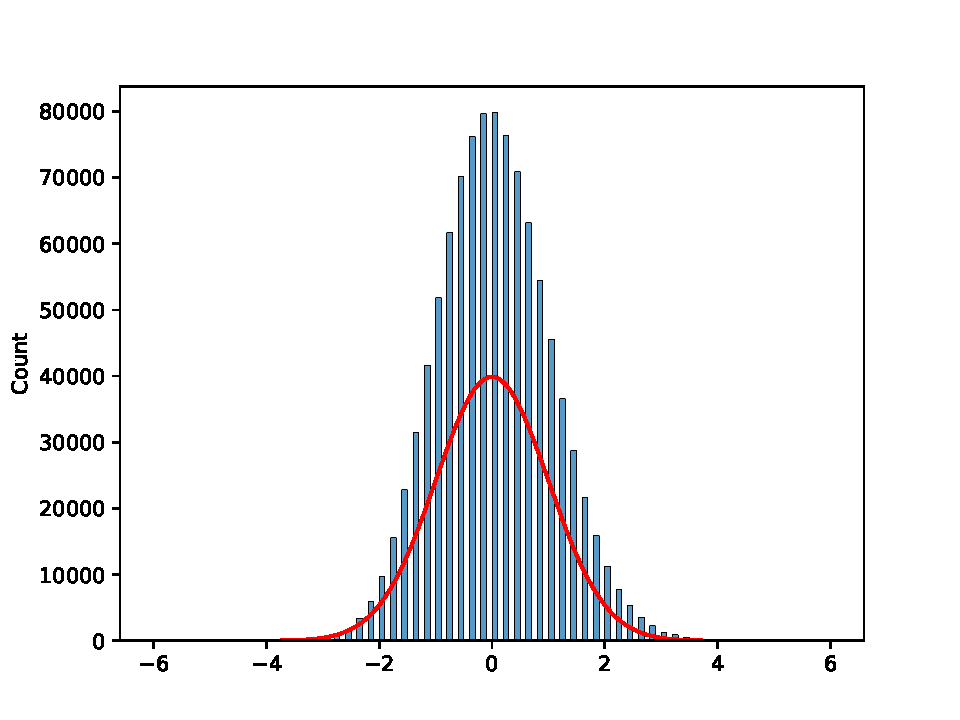
\includegraphics[width = 0.45\textwidth]{../pictures/resfigure_P(5)_size5.pdf}}
    \subfigure[\footnotesize$m=10$]{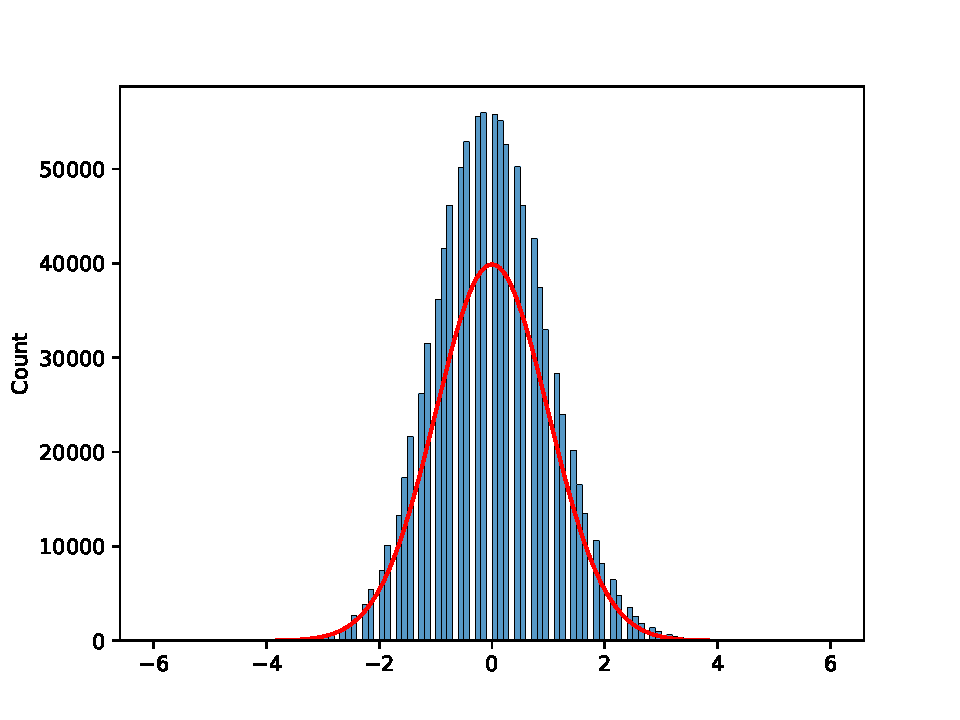
\includegraphics[width = 0.45\textwidth]{../pictures/resfigure_P(5)_size10.pdf}}
    \subfigure[\footnotesize$m=100$]{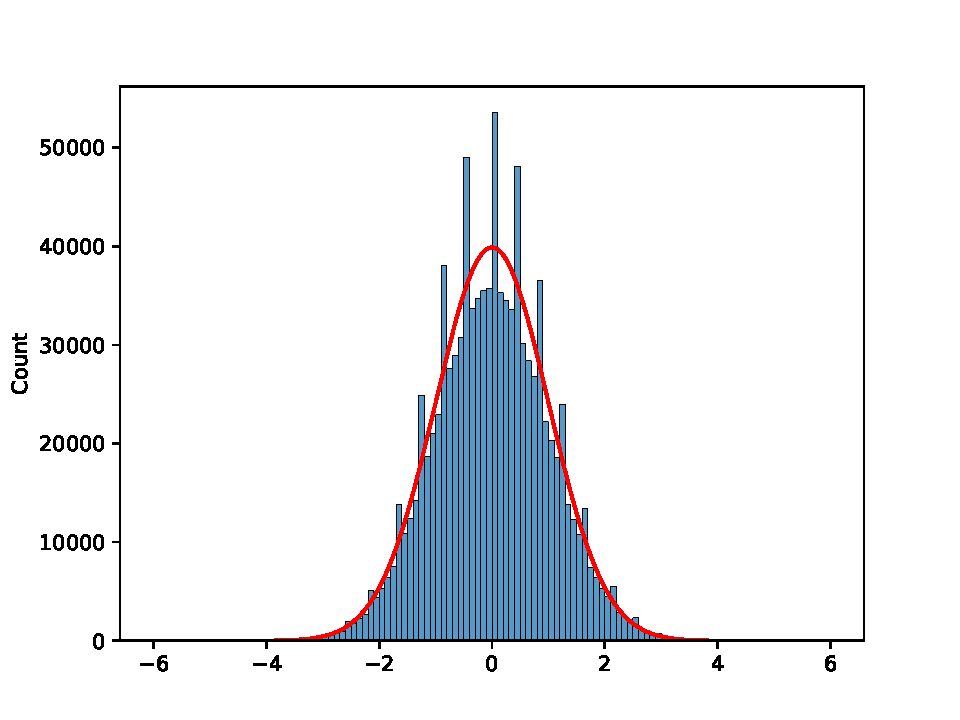
\includegraphics[width = 0.45\textwidth]{../pictures/resfigure_P(5)_size100.pdf}}
    \subfigure[\footnotesize$m=1000$]{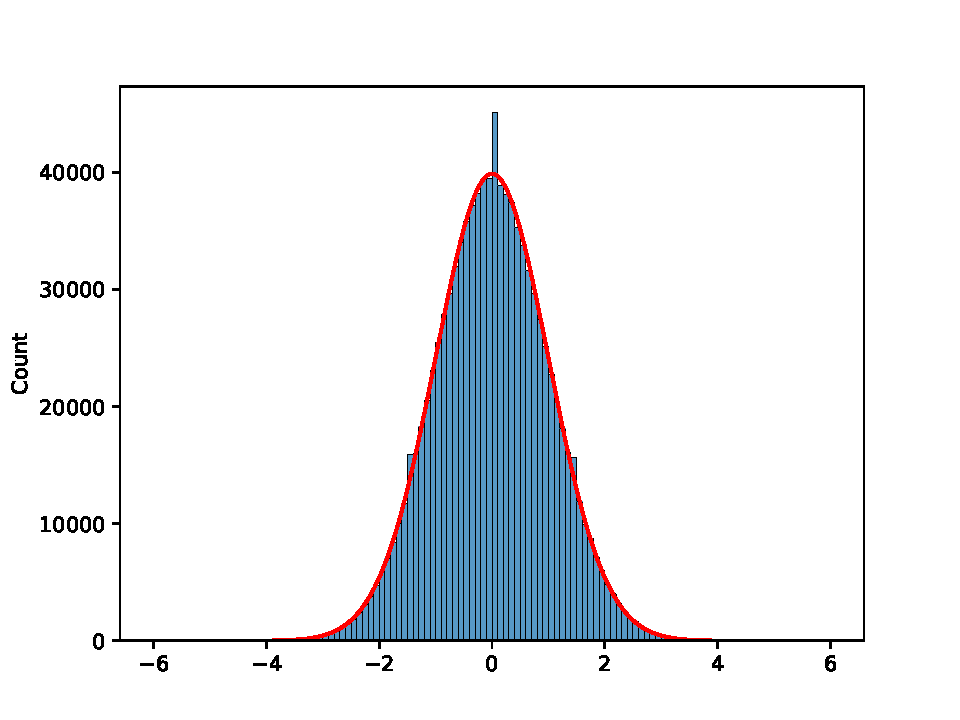
\includegraphics[width = 0.45\textwidth]{../pictures/resfigure_P(5)_size1000.pdf}}
    \caption{\textbf{泊松分布下不同$m$值对应的频数分布直方图,红色曲线代表其在标准正态分布下的理想值}}
    \label{poi}
    \end{figure}
\subsubsection{指数分布}
参数设置:
\[
n=1000000, \lambda = 0.1, \mu = 10, \sigma = 10
\]
实验结果:

画出$m = 1, m = 2, m = 5, m = 10, m = 100, m = 1000$时的频数分布直方图(如图\ref{exp}),从图中可以直观地看到,随着$m$值的升高,$Y$的频数分布直方图不断地拟合接近标准正态分布的理想值。
\begin{figure}[h]

    \subfigure[\footnotesize$m=1$]{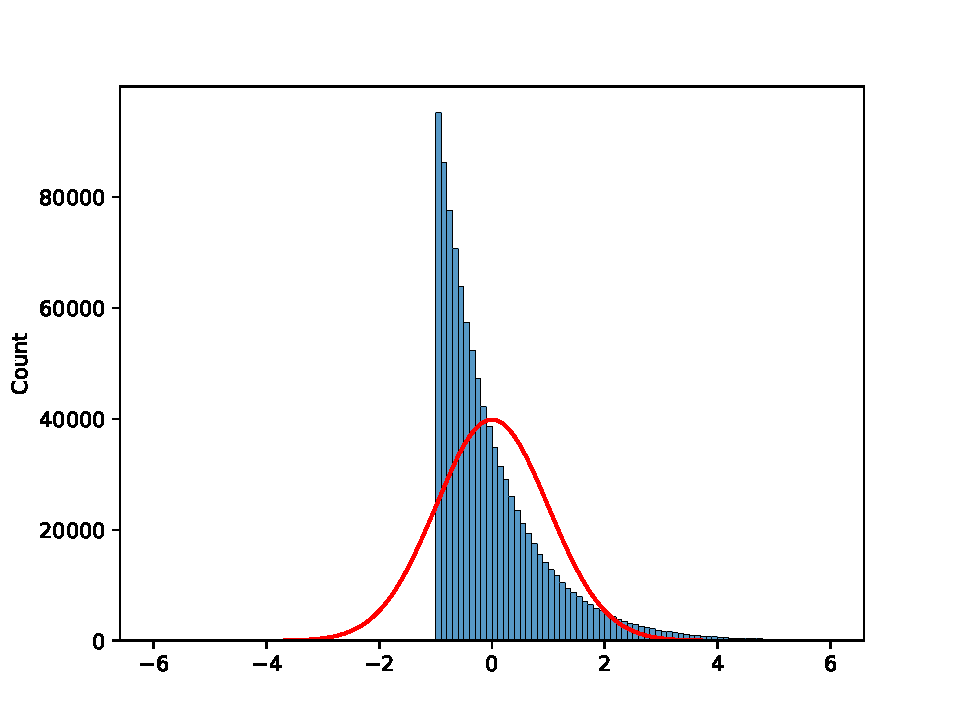
\includegraphics[width = 0.45\textwidth]{../pictures/resfigure_E(0.1)_size1.pdf}}
    \subfigure[\footnotesize$m=2$]{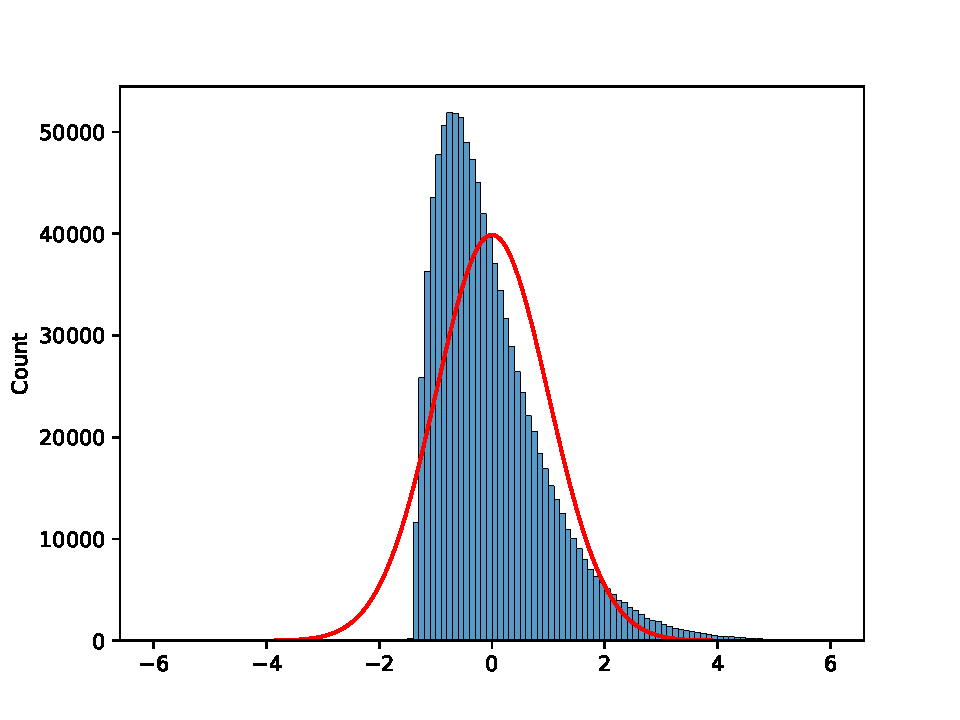
\includegraphics[width = 0.45\textwidth]{../pictures/resfigure_E(0.1)_size2.pdf}}
    \subfigure[\footnotesize$m=5$]{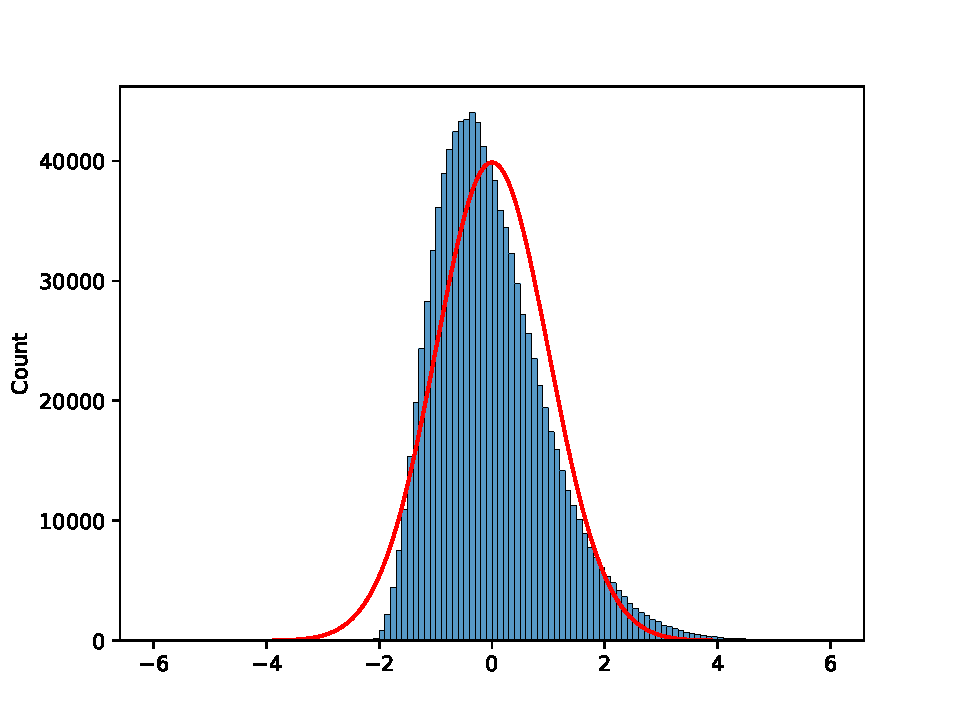
\includegraphics[width = 0.45\textwidth]{../pictures/resfigure_E(0.1)_size5.pdf}}
    \subfigure[\footnotesize$m=10$]{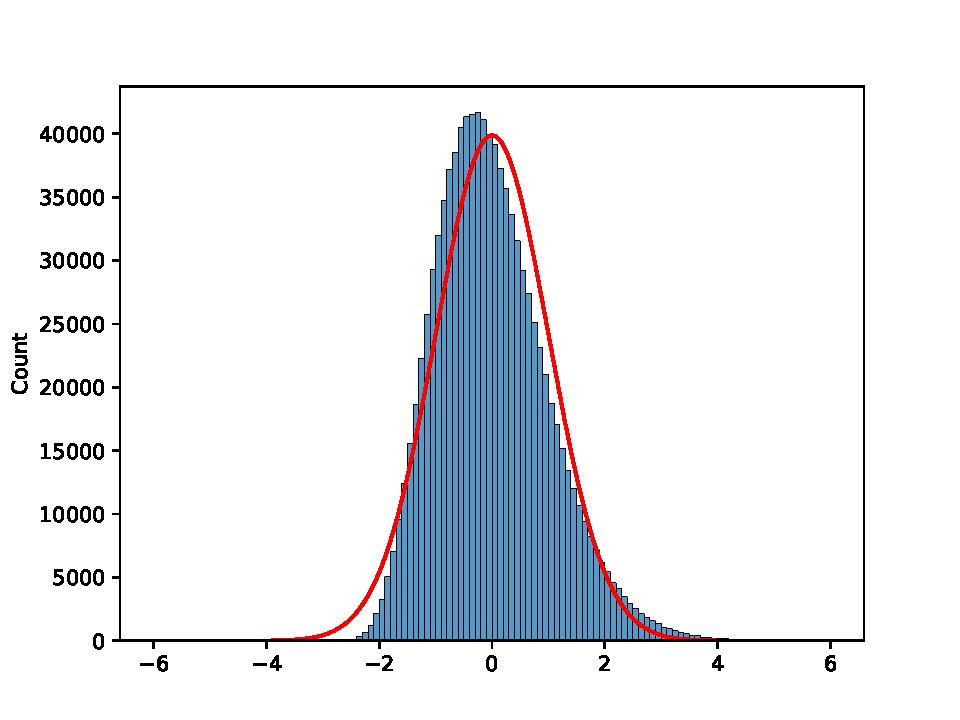
\includegraphics[width = 0.45\textwidth]{../pictures/resfigure_E(0.1)_size10.pdf}}
    \subfigure[\footnotesize$m=100$]{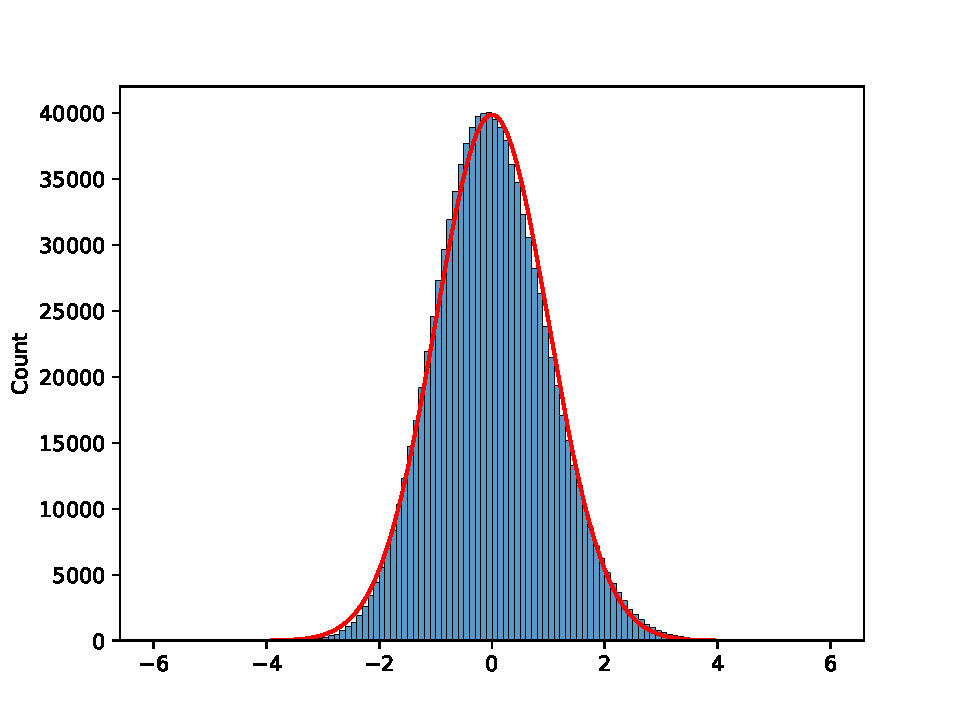
\includegraphics[width = 0.45\textwidth]{../pictures/resfigure_E(0.1)_size100.pdf}}
    \subfigure[\footnotesize$m=1000$]{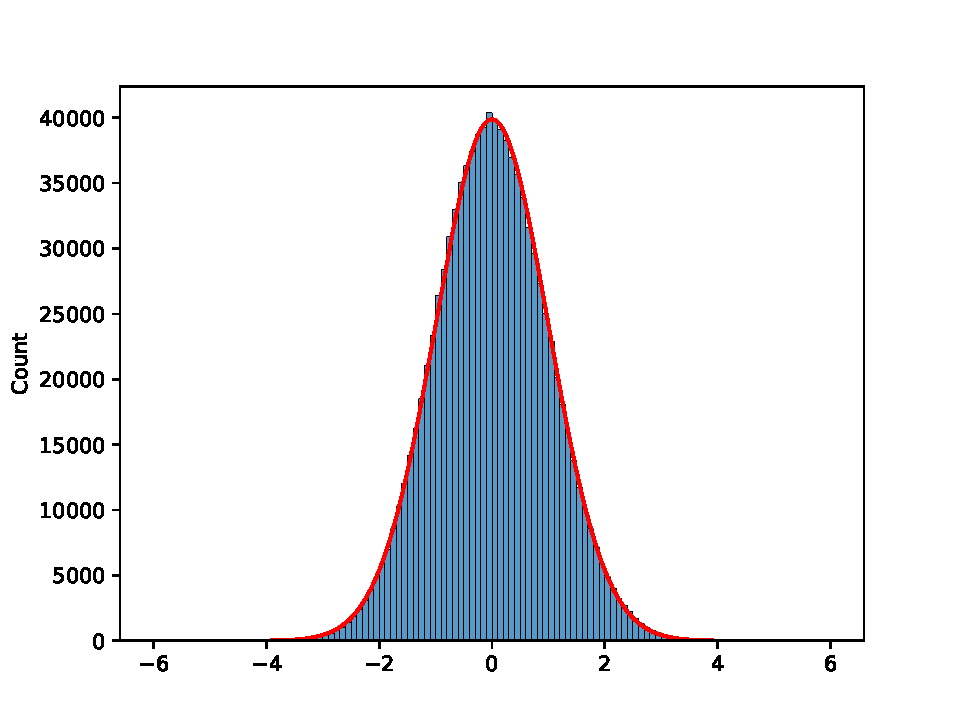
\includegraphics[width = 0.45\textwidth]{../pictures/resfigure_E(0.1)_size1000.pdf}}
    \caption{\textbf{指数分布下不同$m$值对应的频数分布直方图,红色曲线代表其在标准正态分布下的理想值}}
    \label{exp}
    \end{figure}
\subsection{不同随机分布下拟合精度升高的速度}
图\ref{res}中记录了几种不同的随机分布的$Loss$值随着m值的升高的变化。从图中可知:
\begin{itemize}
    \item 连续随机分布:对于指数分布、均匀分布两种随机分布来说,可以观察到两者的Loss曲线呈现较为稳定的下降,当m值较小、Loss值较高时,Loss值下降较快,拟合精度升高的更快。同时均匀分布的Loss值整体更低,在相同的有限m值时拟合效果更好。
    \item 离散型随机分布:对于伯努利分布、泊松分布来说,由于两种随机分布为离散型随机分布,而标准正态分布是连续型随机分布,因此实际数据的逐渐拟合不但体现在y轴上,而且体现在x轴上,因此我们在Loss值曲线中可以观察到的明显的周期性波动,就是在x轴上逐渐拟合的表现。对于Loss值较大的周期性波动,在文章第\ref{discuss}部分会进行讨论。同时,可以观察到伯努利分布较泊松分布更为稳定。
\end{itemize}


\begin{figure}[h]
    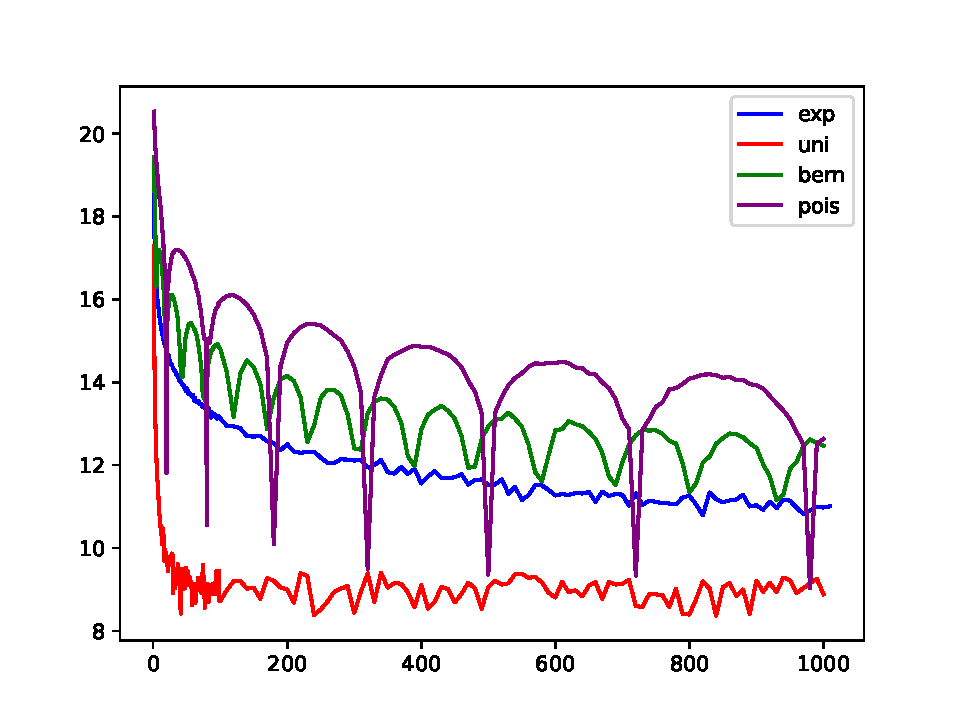
\includegraphics[width=\textwidth]{../data/lossLines.pdf}
    \caption{\textbf{几种不同的随机分布的$Loss$值随着m值的升高的变化}}
    \label{res}
\end{figure}

\section{总结与展望}\label{discuss}
在文章中我们提出了拟合损失函数Loss对于中心极限定理的拟合精度进行描述,并且进行了一系列实验,在不同的随机分布上验证了中心极限定理,同时对于不同的m值测出了Loss值的下降情况。(具体见文章的第\ref{experiment}部分)

研究结果表明,对于连续型随机分布,可以观察到两者的Loss曲线呈现较为稳定的下降;然而对于离散型随机分布,数据呈现周期性的较大波动,具体观察不同的损失函数,可以发现此种随机分布是由于部分区间的实验值的数量为0导致。在后续的文章中,可以继续提出全新的指标函数,从而排除这种扰动,使得指标变化更加平稳,用于更好地描述离散型随机分布的拟合表现。

最后,我们对于Loss值的下降曲线进行观察:连续型随机分布的下降曲线,显然符合$\lim_{m\to+\infty}Loss=0$的表现;对于离散型随机分布,虽然会有周期性的波动,但是这样的波动随着$m$值的增大而减小,因此也符合$\lim_{m\to+\infty}Loss=0$的表现。由此可以再一次用实验量化的证明中心极限定理。显然,我们可以继续增加$m$值,从而观察到最终$Loss$趋近于0。

\bibliography{references}

\end{document}